\documentclass[11pt,a4paper]{article}

\usepackage[margin=2.2cm]{geometry}
\usepackage{fontspec}
\usepackage{luatexja-fontspec}

% System-installed TrueType fonts — no reliance on broken lmodern type1 metrics
\setmainfont{DejaVu Serif}[
  BoldFont = DejaVu Serif Bold,
  ItalicFont = DejaVu Serif Italic,
  BoldItalicFont = DejaVu Serif Bold Italic,
  Scale = 0.94]
\setsansfont{DejaVu Sans}[Scale = 0.92]
\setmonofont{DejaVu Sans Mono}[Scale = 0.88]

% CJK font — Droid Sans Fallback covers all the Chinese we need
\usepackage{luatexja}
\setmainjfont{Droid Sans Fallback}
\setsansjfont{Droid Sans Fallback}

\usepackage{graphicx}
\usepackage{longtable}
\usepackage{booktabs}
\usepackage{array}
\usepackage{xcolor}
\usepackage{fancyvrb}
\usepackage[hidelinks]{hyperref}
\usepackage{enumitem}
\setlist{nosep, leftmargin=*}

\usepackage{titlesec}
\titleformat{\section}{\Large\bfseries}{\thesection}{0.6em}{}
\titleformat{\subsection}{\large\bfseries}{\thesubsection}{0.6em}{}

\setlength{\parindent}{0pt}
\setlength{\parskip}{0.45em}

\title{\vspace{-1.5cm}\textbf{Selective Rollout — Gate 实验中文报告}\\[0.2em]
\large \textbf{最终结论：通过}\\[0.1em]
\small Qwen2.5-7B-Instruct · ALFWorld · N=100, G=8}
\author{}
\date{}

\begin{document}
\maketitle
\vspace{-1.5em}

\begin{quote}
\textbf{一句话}：Rollout 中途第 K=10--15 步的动作 divergence 能预测最终 reward variance，Spearman $\rho$ 最高 \textbf{0.42}（p=1.4$\times 10^{-5}$），AUROC 最高 \textbf{0.77}。信号足够强，值得把 per-group early termination 做进正式 project。
\end{quote}

\section{实验配置}

\begin{itemize}
  \item \textbf{环境}：ALFWorld（TextWorld 后端），混合 6 种任务类型。
  \item \textbf{模型}：Qwen2.5-7B-Instruct，单 VLLM engine，temperature 0.7。
  \item \textbf{任务数}：valid\_seen 切分里随机抽 100 个（seed=42）。
  \item \textbf{组大小 G}：每个任务并行采 8 条 trajectory（同一初始状态，独立采样）。
  \item \textbf{Max steps}：30。
  \item \textbf{耗时}：单张 RTX 6000 Ada 上 45 分钟跑完，零失败。
\end{itemize}

\textbf{100 个 group 的结果分布}：

\begin{itemize}
  \item 全败（reward 0/8）：\textbf{25} 组
  \item 混合（非零方差）：\textbf{61} 组
  \item 全胜（reward 8/8）：\textbf{14} 组
  \item 零方差比例：\textbf{39\%}（25+14）
\end{itemize}

如果能在 step=10 完美识别出零方差组，理论可节省的 rollout 算力
$\approx 39/100 \times (30-10)/30 \approx$ \textbf{26\%}。

\section{核心数字}

\begin{longtable}{@{}clllll@{}}
\toprule
排名 & K & divergence 指标 & Spearman $\rho$ & p-value & AUROC \\
\midrule
1 & 15 & prefix\_edit\_distance\_mean    & \textbf{0.419} & $1.4\times 10^{-5}$ & 0.773 \\
2 & 20 & prefix\_edit\_distance\_mean    & 0.418 & $1.5\times 10^{-5}$ & 0.753 \\
3 & 10 & action\_bigram\_jaccard\_mean   & 0.407 & $2.7\times 10^{-5}$ & 0.770 \\
4 & 15 & action\_bigram\_jaccard\_mean   & 0.406 & $2.8\times 10^{-5}$ & 0.752 \\
5 & 10 & unique\_prefix\_ratio           & 0.398 & $4.0\times 10^{-5}$ & 0.751 \\
\bottomrule
\end{longtable}

Gate 标准（$|\rho| \geq 0.4$ 或 $2 \times (\text{AUROC}-0.5) \geq 0.4$）：28 个
(metric $\times$ K) 组合中有 \textbf{5 个通过}。

\section{信号在哪里：K=10--15 是 sweet spot}

$\rho$ / AUROC 双指标网格（详见 figures/heatmap\_rho\_auroc.png）：

\begin{longtable}{@{}lllll@{}}
\toprule
指标 $\backslash$ K & 5 & 10 & 15 & 20 \\
\midrule
unique\_action\_ratio         & 0.31 / 0.70 & \textbf{0.38 / 0.75} & 0.27 / 0.64 & 0.17 / 0.58 \\
unique\_prefix\_ratio         & 0.32 / 0.70 & \textbf{0.40 / 0.75} & 0.31 / 0.67 & 0.21 / 0.61 \\
action\_bigram\_jaccard\_mean & 0.29 / 0.69 & \textbf{0.41 / 0.77} & \textbf{0.41 / 0.75} & 0.39 / 0.72 \\
prefix\_edit\_distance\_mean  & 0.25 / 0.66 & 0.37 / 0.76 & \textbf{0.42 / 0.77} & \textbf{0.42 / 0.75} \\
obs\_unique\_ratio            & 0.25 / 0.66 & 0.40 / 0.75 & 0.31 / 0.66 & 0.09 / 0.53 \\
action\_entropy               & 0.29 / 0.70 & \textbf{0.37 / 0.74} & 0.26 / 0.64 & 0.16 / 0.57 \\
termination\_fraction         & $-0.19$ / 0.45 & $-0.06$ / 0.51 & 0.11 / 0.56 & 0.16 / 0.59 \\
\bottomrule
\end{longtable}

（格式：$\rho$ / AUROC）

\begin{itemize}
  \item \textbf{K=5 太早}：大部分 trajectory 还在跑开头那几个固定动作（go to cabinet 1 之类），还没拉开差距。
  \item \textbf{K=10--15 最优}：8 条 trajectory 已经显露出各自的"意图"，同时距离终点还远，gate 的边际收益最大。
  \item \textbf{K=20 信号仍存}，但代价也上来了（距离 30 步的 max 已经跑了 2/3）。
  \item \textbf{termination\_fraction 单独用没用}：全胜组早早结束、全败组根本不结束，两类零方差在这维度上往相反方向拉。
\end{itemize}

\begin{center}
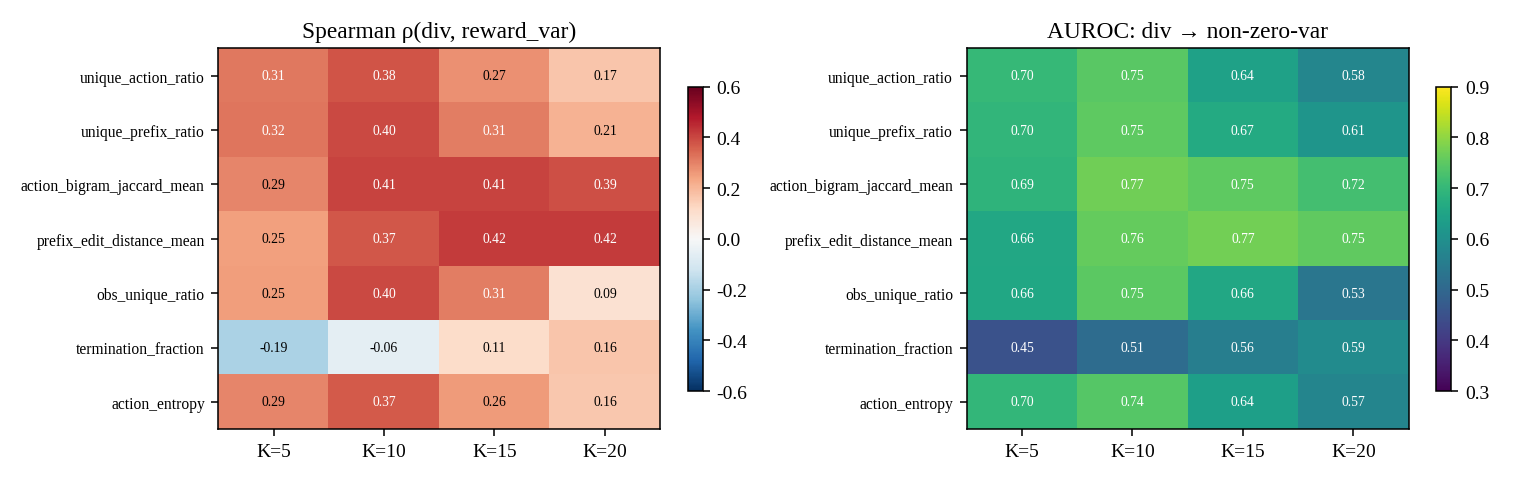
\includegraphics[width=\linewidth]{figures/heatmap_rho_auroc.png}
\end{center}

\section{发现了一个不对称性}

按 group 最终结果分三类做的 stratified scatter：

\begin{itemize}
  \item \textbf{全胜组（n=14）}：紧紧聚集在\textbf{低 divergence}（基本 $\leq$ 0.3）。模型知道怎么做时，8 条采样收敛一致 —— 容易识别。
  \item \textbf{混合组（n=61）}：分散在\textbf{中到高 divergence}（0.1--0.85），中心约 0.5。和全胜组分离明显。
  \item \textbf{全败组（n=25）}：分散在\textbf{整个范围}（0.0--0.75）。模型有时锁步地犯同样的错（低 div），有时混乱地各自瞎撞（高 div，但还是没人赢）。
\end{itemize}

\begin{center}
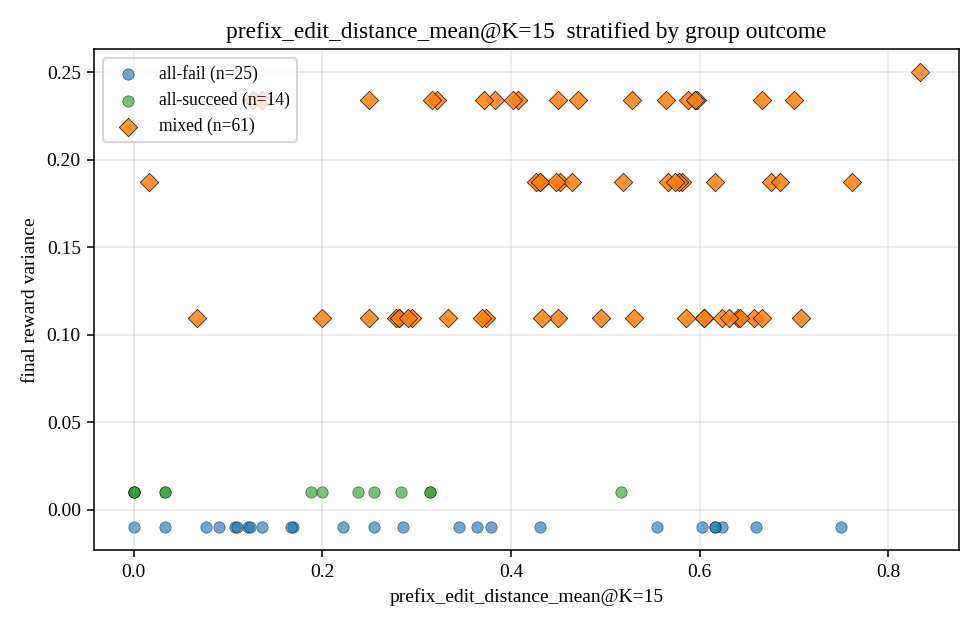
\includegraphics[width=0.95\linewidth]{figures/stratified_prefix_edit_distance_mean_K15.png}
\end{center}

\textbf{对 per-group early termination 的含义}：

\begin{itemize}
  \item 容易砍的零方差组 \#1：\textbf{正在收敛到成功}（低 div $\Rightarrow$ 8 条采样基本一致，稳）。
  \item 容易砍的零方差组 \#2：\textbf{协调地在犯错}（低 div，8 条都在同一个错误路径上）。
  \item 最难识别：\textbf{高 div 的全败组} —— 它们看起来就像非零方差的混合组。这类只能用 DAPO 那种事后 filter，early termination 救不了。
\end{itemize}

建议正式版用\textbf{双阈值 gate}：``div@15 $<$ 0.10 \textbf{或} div@15 $>$ 0.75 $\Rightarrow$ 提前终止''，两端通吃。

\section{按任务类型看}

每个任务类型内部的最佳信号（correlation\_by\_task\_type.csv）：

\begin{longtable}{@{}lcclcll@{}}
\toprule
task\_type & n & 最佳 K & 最佳 metric & $\rho$ & AUROC \\
\midrule
look\_at\_obj\_in\_light         &  8 & 15 & unique\_prefix\_ratio    & \textbf{0.810} & \textbf{1.000} \\
pick\_two\_obj\_and\_place       & 20 & 20 & termination\_fraction    & \textbf{0.788} & 0.857 \\
pick\_cool\_then\_place\_in\_recep  & 19 & 20 & termination\_fraction    & 0.730 & 0.821 \\
pick\_and\_place\_simple         & 24 & 15 & unique\_action\_ratio    & 0.688 & 0.857 \\
pick\_heat\_then\_place\_in\_recep  & 11 & 10 & action\_entropy          & 0.546 & \textbf{1.000} \\
pick\_clean\_then\_place\_in\_recep & 18 & 15 & termination\_fraction    & 0.457 & 0.708 \\
\bottomrule
\end{longtable}

\textbf{6 个任务类型上信号都稳}（最低 AUROC 0.71，中位数 0.86）。但\textbf{每类最佳指标不同} —— 说明 task-aware gate（针对任务类型选 K 和 metric）会比单一全局阈值更强。

\section{具体例子}

\subsection*{典型"该砍"的零方差组（低 div + 全胜）}

任务：\texttt{pick\_and\_place\_simple} —— 8/8 成功，div@10 = 0.000

\begin{Verbatim}[fontsize=\small,frame=single]
traj 0: go to cabinet 1 | open cabinet 1 | go to cabinet 2 | ...
traj 1: go to cabinet 1 | open cabinet 1 | go to cabinet 2 | ...
...   (8 条前 10 步完全相同，最后全胜)
\end{Verbatim}

$\Rightarrow$ 到 step 10 就已经能判定这组对梯度贡献为零。\textbf{提前砍}。

\subsection*{典型"该留"的非零方差组（高 div + 混合）}

任务：\texttt{look\_at\_obj\_in\_light} —— 5/8 成功，div@10 = 0.748

\begin{Verbatim}[fontsize=\small,frame=single,breaklines=true]
traj 0: go to bed 1 | go to desk 1 | go to sidetable 1 | use desklamp 1 | ...
traj 3: go to bed 1 | take pillow 1 from bed 1 | go to desk 1 | look | ...
traj 7: go to bed 1 | take pillow 1 from bed 1 | go to sidetable 1 | go to sidetable 2 | ...
\end{Verbatim}

$\Rightarrow$ 8 条 trajectory 分化成不同的探索策略 $\Rightarrow$ 最终有胜有败 $\Rightarrow$ \textbf{8 条全留}。

\subsection*{Gate 失败的边缘 case}

任务：\texttt{pick\_and\_place\_simple} —— 3/8 成功，div@10 = 0.000

\begin{Verbatim}[fontsize=\small,frame=single]
(8 条前 10 步完全相同，到 step 10 之后才分化成不同的终局动作)
\end{Verbatim}

$\Rightarrow$ 如果在 K=10 判定，会误判为零方差提前砍掉。
\textbf{修法}：用 K=15 或 20；或者按任务类型 task-aware 地选 K。

\section{结论}

\textbf{可以做正式 project。} 信号统计显著（p $< 10^{-4}$），方向与假设一致，绝对值也足够强（$|\rho| \approx 0.42$，AUROC $\approx 0.77$）。建议把 per-group early-termination 做进 GRPO 的 rollout 循环。前面发现的不对称性说明，生产版的 gate 应当是双阈值 —— 低 div 和高 div 两端都砍。

\subsection*{下一步（超出本 gate 实验的范围）}

\begin{enumerate}
  \item WebShop 上验证泛化性（agent-native 的信号应当能迁移；math 没有这种结构）。
  \item G=16 看 divergence 度量会不会更稳定。
  \item 真正把 early-termination 接进 verl/GRPO 的 rollout 闭环，量化：节省多少算力 vs 梯度范数下降多少。
  \item Task-aware K 选择：根据任务类型挑选最优 (metric, K) 组合。
\end{enumerate}

\section{产物清单}

\begin{itemize}
  \item \texttt{data/rollouts.jsonl} —— 100 组 $\times$ 8 轨迹的原始 rollout 数据（可复现）
  \item \texttt{data/metrics.parquet} —— 每组的 divergence metrics $\times$ K
  \item \texttt{results/correlation\_table.csv} —— Spearman $\rho$ + AUROC 表
  \item \texttt{results/correlation\_by\_task\_type.csv} —— 按任务类型拆分的相关性
  \item \texttt{results/figures/heatmap\_rho\_auroc.png} —— (metric $\times$ K) 双指标热力图
  \item \texttt{results/figures/stratified\_prefix\_edit\_distance\_mean\_K15.png} —— 三分层散点
  \item \texttt{results/figures/hist\_zero\_vs\_nonzero.png} —— 零方差 vs 非零方差的 div 分布对比
  \item \texttt{results/figures/scatter\_K\{5,10,15,20\}.png} —— 各 K 下所有 metric 的散点矩阵
  \item \texttt{results/report.md} / \texttt{results/report\_zh.md} —— 英文 / 中文报告（Markdown）
\end{itemize}

\end{document}
